\documentclass[12pt,a4paper]{article}
\usepackage[utf8]{inputenc}
\usepackage{amsmath}
\usepackage{graphicx}
\usepackage{multicol}
\usepackage{hyperref}
\usepackage{cite}
\usepackage{float}

\title{Alternate Splicing: The Mechanism of Protein Diversification}
\author{Mara-Andreea Spataru, Grupa 341}
\date{\today}

\begin{document}
	
	\maketitle
	
	\begin{multicols}{2}
		\section{Introduction}
		Alternate Splicing is an essential process for the eukaryotic genes, the reason is because it lets a single DNA segment code for multiple proteins. This mechanism has a significant contribution to protein diversity and to the functional complexity of organisms.
		
		\section{Exons and Introns}
		To get a better understanding of how alternate splicing works, we must first have a clear definition for exons and introns. Exons are DNA sequences that contain the necessary information to synthesize proteins, whilst the introns are non-coding sequences which must be eliminated to produce a mature messenger RNA (mRNA). This process in which introns are eliminated and exons are reunited is called splicing.
		
		
		\section{How Does Alternate Splicing Happens?}
		Alternate splicing lets cells eliminate introns and combine exons in numerous ways, thus generating multiple versions of mature mRNA. This process takes place in the presence of a molecular complex named spliceosome, which recognizes and processes the specific sequences of the pre-mRNA (this is the primary transcript in the transcription process). The way in which the exons are combined influences the structure and function of the protein that results.
		
		\section{Different Types of Alternate Splicing}
		There are many types of alternate splicing:
		\begin{itemize}
			\item Exon skipping: An exon is omitted from the final mRNA, which results in the production of a different protein.
			\item Alternative use of 5' or 3' splice sites: The use of alternative splice sites at 5' or 3' end of the exon, thus modifying its length.
			\item Intron retention: An intron is kept in the mature mRNA, thus influencing the function of the resulting protein.
			\item Mutually exclusive exons: Two exons are alternatively included, but never both(either one or the other) in the same mRNA.
		\end{itemize}
		
		\section{Biological Significance}
		Alternate splicing has a crucial role in protein diversification, letting organisms generate a large range of functional proteins all starting with a limited number of genes. This process is essential in cellular differentiation and development.
		
		\section{Clinical Implications}
		Some anomalies can appear due to alternate splicing, and these can lead to some illnesses, including cancer or neurodegenerative diseases.
		
		\section{Regulation of Alternate Splicing}
		The process of alternate splicing is not made at random, but it is controlled by many factors that decide how the RNA sections are chosen to be kept for the final version of the genetic message. Some of the factors that hold the greatest importance are:
		\begin{itemize}
			\item Proteins that help or block the splicing: some proteins attach themselves to the RNA and influence how its segments are combined by determining which exons are kept and which are eliminated.
			\item Different signals inside RNA: Processed RNA contains some instructions in its structure that guide to eliminate and unite some parts in a specific way.
			\item Chemical changes in DNA: Changes like methylation (the addition of a methyl group on a substrate) can make some regions harder or easier to be accessed by the splicing process.			
			\item Cell type and external conditions: Some cells may need different versions of the same protein, thus the alternate splicing is adjusted by the cellular type and signals received from the environment. 
		\end{itemize}
		
		\section{Study Methods}
		Modern technologies, like RNA sequencing, allow a global analysis of alternate splicing events. These methods offer detailed information and help in better understanding the role of alternate splicing.
		
	\end{multicols}
	
	%imagine 1 separat de zona cu doua coloane, centrata
	\begin{figure}[t]
		\centering
		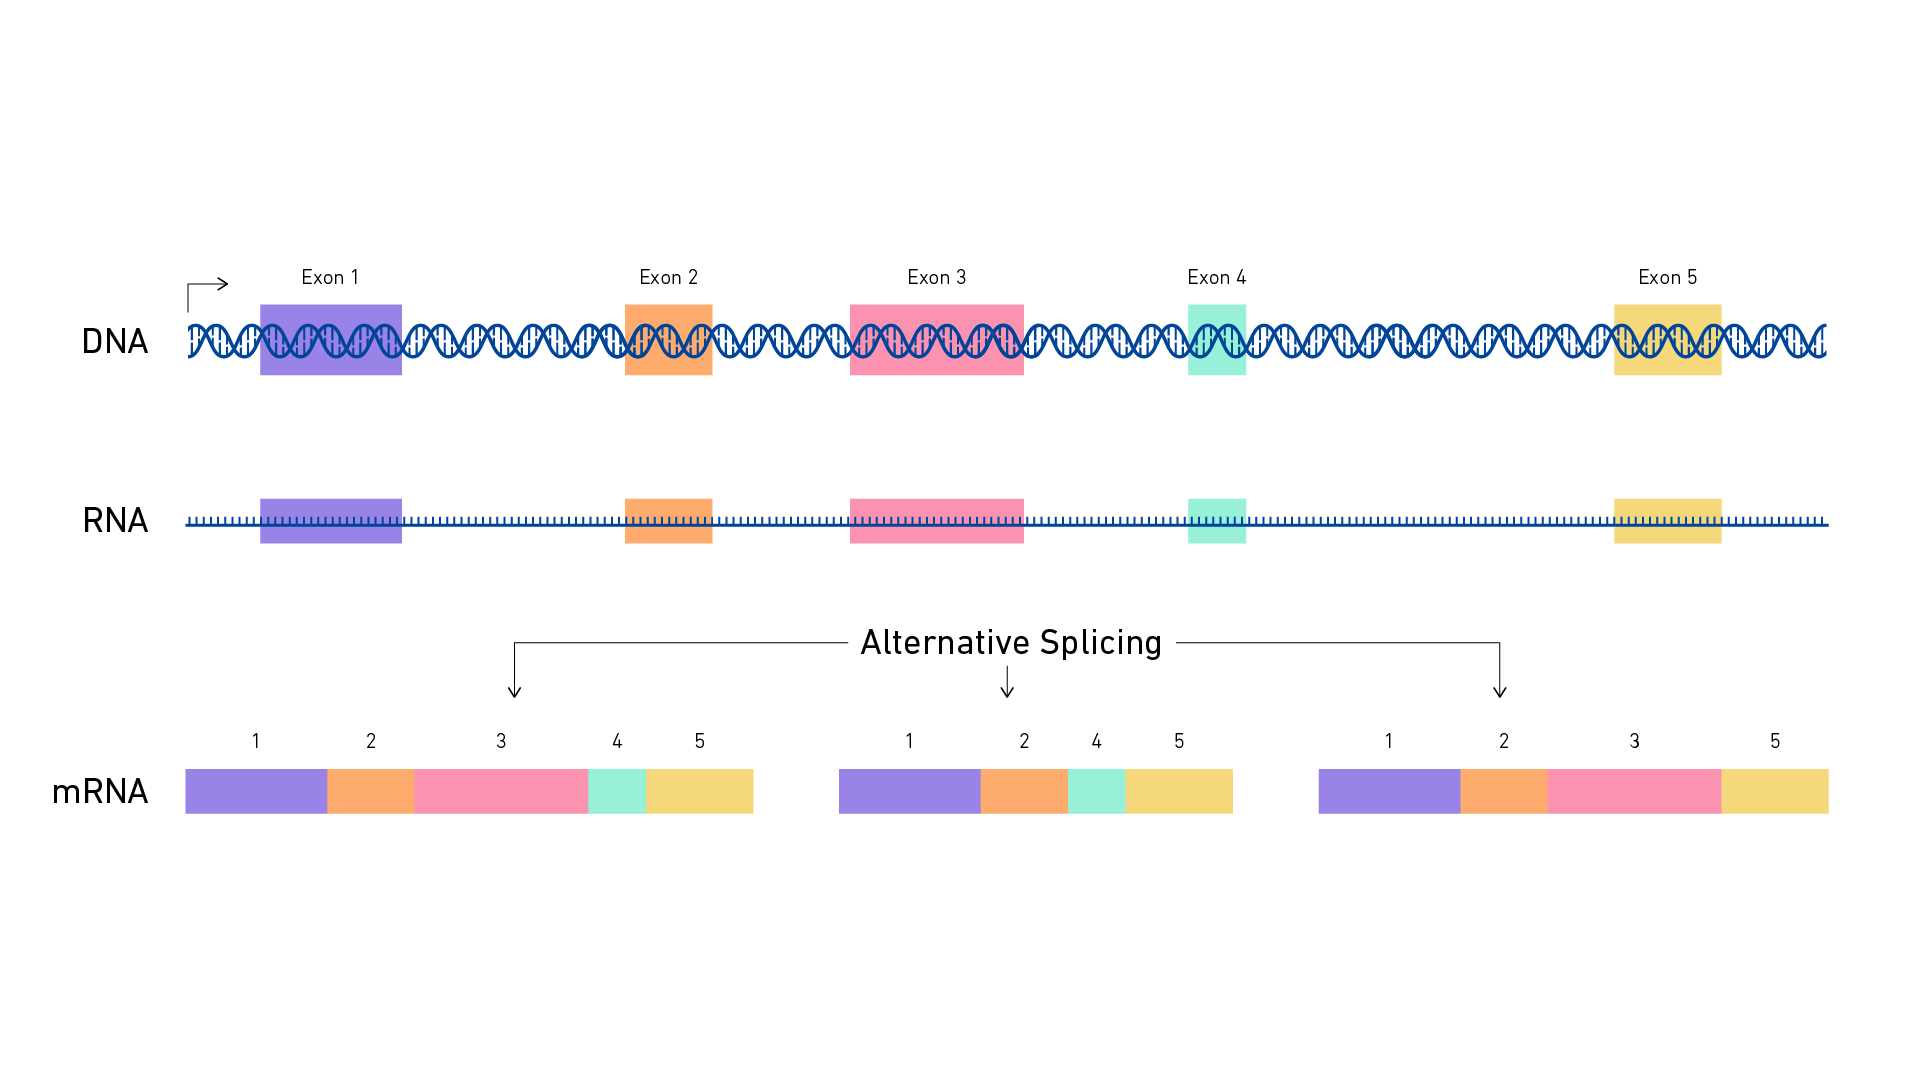
\includegraphics[width=0.8\textwidth]{alternatesplicing1.png}
		\caption{Illustration of the spliceosome process}
		\label{fig:spliceosome}
		\small{Source: Technology Networks (2023). \url{https://www.technologynetworks.com/genomics/articles/alternative-splicing-importance-and-definition-351813}}
	\end{figure}
	
	%\newpage
	
	\begin{multicols}{2}
		\section{Conclusion}
		Alternate splicing is a fundamental mechanism that extends the informational capacity of the genome, allowing organisms to generate protein diversity, which is needed for the complex biological functions and for adapting to different environments. Understanding this process helps offering new and important perspectives about molecular biology and the mechanisms that lie at the core of multiple human diseases. 
		
		%imaginea 2 centrata la coloana
		\begin{figure}[H]
			\centering
			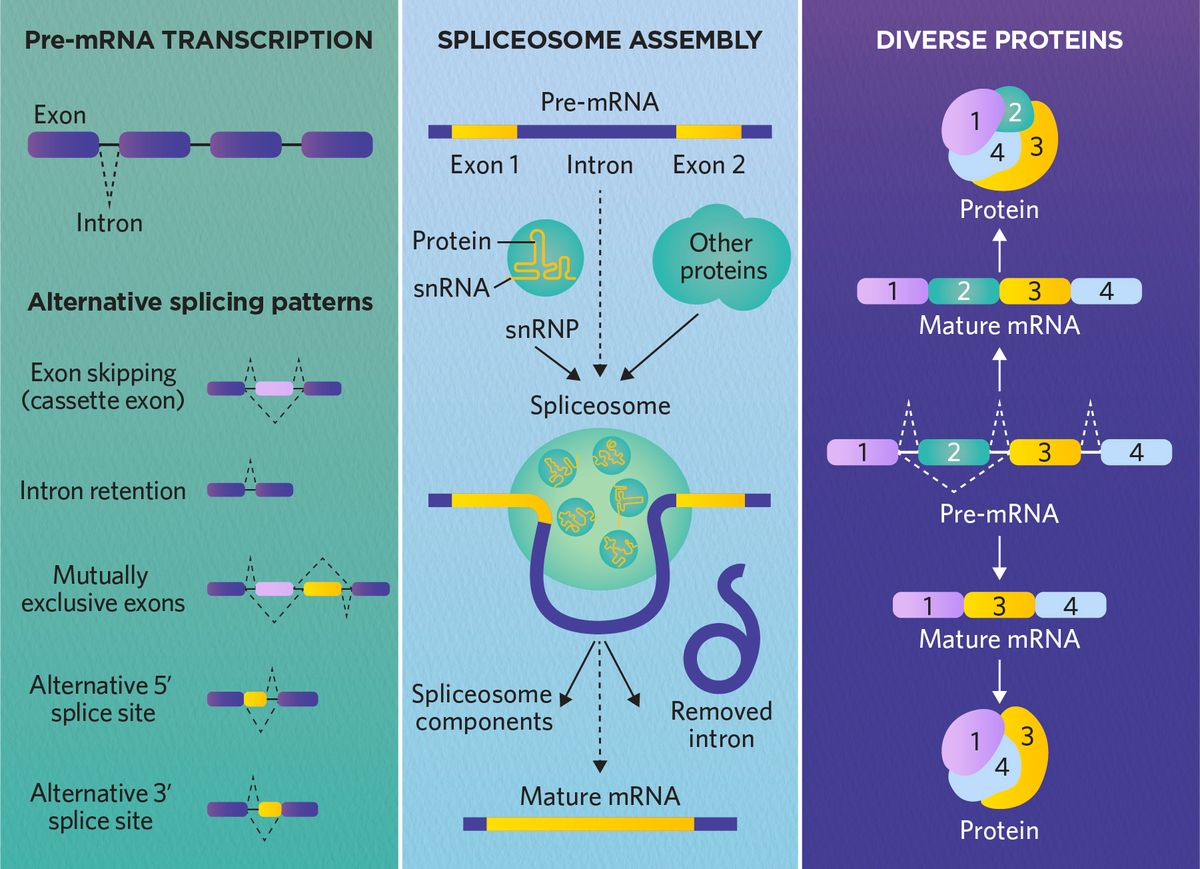
\includegraphics[width=0.8\linewidth]{alternatesplicing2.jpg}
			\caption{Alternate splicing types diagram}
			\label{fig:alternativesplicing}
			\small{Source: Wikipedia contributors (2023). \url{https://en.wikipedia.org/wiki/Alternative_splicing}}
		\end{figure}
	\end{multicols}
	
	%Bbiliografie folosind APA style
	\newpage
	\section*{Bibliography}
	\begin{enumerate}
		\item Black, D. L. (2003). Mechanisms of alternative pre-messenger RNA splicing. \textit{Annual Review of Biochemistry}, 72, 291-336. ANNUALREVIEWS.ORG.
		\item Nilsen, T. W., \& Graveley, B. R. (2010). Expansion of the eukaryotic proteome by alternative splicing. \textit{Nature}, 463(7280), 457-463. NATURE.COM.
		\item Wang, E. T., et al. (2008). Alternative isoform regulation in human tissue transcriptomes. \textit{Nature}, 456(7221), 470-476.
		\item Baralle, F. E., \& Giudice, J. (2017). Alternative splicing as a regulator of development and tissue identity. \textit{Nature Reviews Molecular Cell Biology}, 18(7), 437-451.
		\item Braunschweig, U., et al. (2014). Widespread intron retention in mammals leads to nonsense-mediated mRNA decay. \textit{Genome Research}, 24(3), 824-835.
		\item Technology Networks. (2023). \href{https://www.technologynetworks.com/genomics/articles/alternative-splicing-importance-and-definition-351813}{Alternative Splicing: Importance and Definition}.
		\item Wikipedia contributors. (2023). \href{https://en.wikipedia.org/wiki/Alternative_splicing}{Alternative splicing}.
		\item National Human Genome Research Institute. (2023). \href{https://www.genome.gov/genetics-glossary/Alternative-Splicing}{Alternative Splicing}.
	\end{enumerate}
	
\end{document}